%========================================================================================
% TU Dortmund, Informatik Lehrstuhl VII
%========================================================================================

\chapter{Vom Höchstspannungsnetz zum Graphen}
\label{Kapitel 2}
%


\section{Graph}
\label{Graph}
%
Ein Graph ist eine Struktur, die Informationen über zusammenhängende Objekte repräsentiert. Die jeweiligen Objekte werden Knoten und deren Verbindungen Kanten genannt. 



\section{Höchstspannungsnetz}
\label{Kapitel_2_-_Unterkapitel_1}
%

Um das weitere Vorgehen zu verstehen, ist es wichtig zu wissen wie ein Höchstspannungsnetz aufgebaut ist. Das Höchstspannungsnetz ist eine besondere Form des Stromnetzes. Um über größere Distanzen hinweg Strom verteilen zu können, ist es effektiver dies mit einer höheren Spannung zu tun, daher auch der Name. Denn je höher die verwendete elektrische Spannung, desto geringer ist die Verlustleistung. 

Die Freileitungen führen über Hochspannungsmasten zu den verschiedenen Orten. Über einen Hochspannungsmast können mehrere Leiterseile verteilt werden. Ein Leiterseil dient der eigentlichen Stromübertragung.   


    \begin{figure}[t]
    	\centering
    	{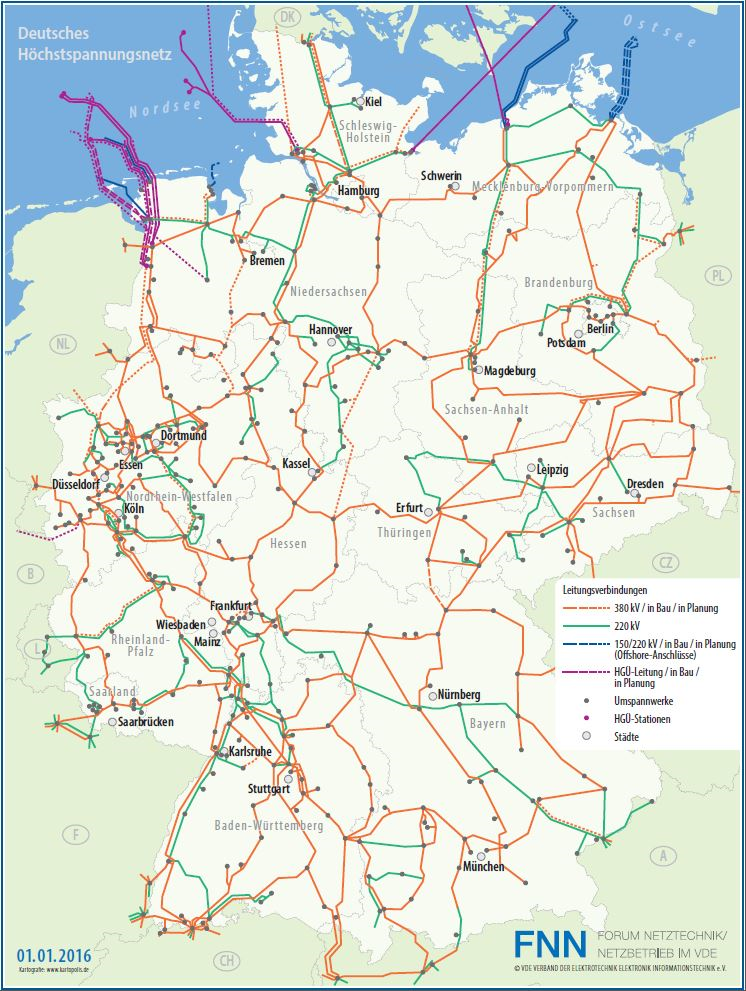
\includegraphics[scale=0.5]{bilder/hochstspannungsnetz}\label{fig_hochstspannungsnetz}
    	}\\
    	\caption[Karte des deutschen Höchstspannungsnetzes]{Karte des deutschen Höchstspannungsnetzes}
    	\label{fig_hochstspannungsnetz2}
    \end{figure}
\section{Kapitel 2 - Unterkapitel 2}
\label{Kapitel_2_-_Unterkapitel_2}
%

Es wurden zwei Schritte unternommen um aus dem Höchstspannungsnetz einen repräsentierenden Graphen zu bekommen. Zum einen wurden die jeweiligen Masten zu Knoten und jeweils eins ihrer Leiterseile zu einer verbindenden Kante. Die Position der Masten war aus einer Karte des Höchstspannungsnetz zu bekommen, ebenso deren Verbindungen. 

Da es besonders wichtig ist darzustellen wie viele einzelne Leiterseile über die jeweiligen Verbindungen laufen, musste dieses noch hinzugefügt werden. Es wurde für jedes Leiterseil welches über einen der Masten lief ein jeweiliger Knoten erstellt, und jeweils mit einer Kante verbunden. Diese zusätzlichen Knoten wurden direkt neben dem ursprünglichen Knoten verteilt. Nun hat man die wichtigsten Informationen des Netzes in einen Graphen übertragen.

Die Städte und Orte werden dabei als unbewegliche Knoten angelegt damit der resultierende Graph nicht zu sehr vom ursprünglichen abweicht. Jegliche Eckpunkte zwischen den Orten wurde mithilfe eines weiteren beweglichen Knotens modelliert.

\begin{figure}[t]
	\centering
	\subfigure[Ausschnit des deutschen Höchstspannungsnetzes. Die markierten Orte werden zu den Knoten und die Verbindungen werden zu den Kanten des Graphen.]
	{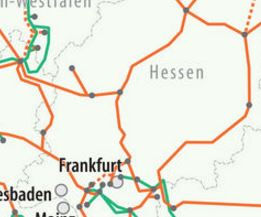
\includegraphics[scale=0.8]{bilder/kartenausschnitt}\label{fig_kartenausschnitt}
	}
	\hspace{1.0cm}%
	\subfigure[Den Ausschnitt der Karte dann als Graphen mit jeweils nur einer Leitung.]
	{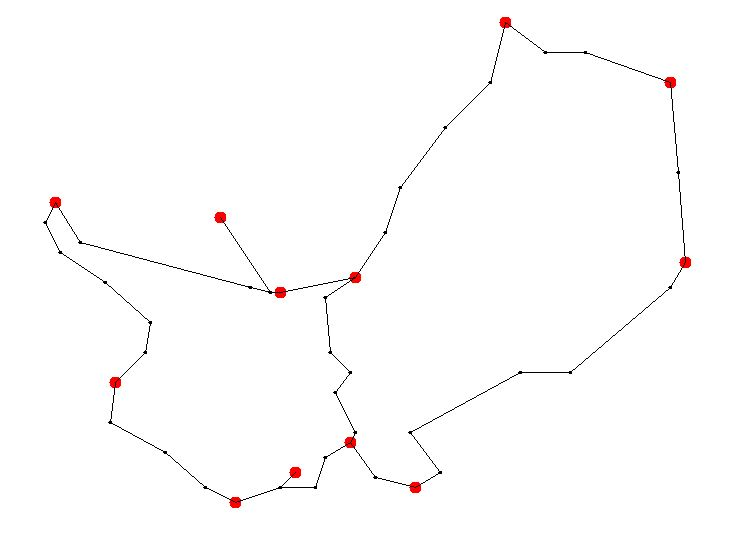
\includegraphics[scale=0.4]{bilder/ausschnittgraph}\label{fig_ausschnittgraph}
	}
	\hspace{1.0cm}%
	\subfigure[Die zusätzlichen Leitungen wurden neben dem eigentlichen Knoten hinzugefügt. Hier jeweils immer genau drei.]
	{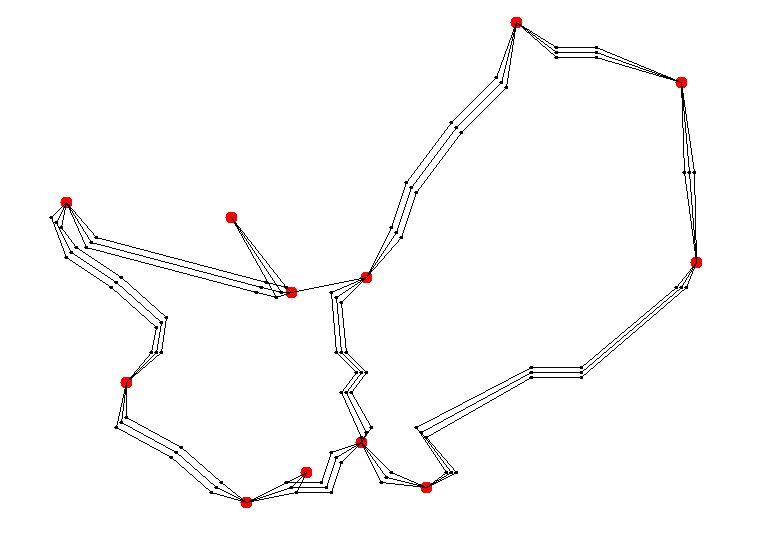
\includegraphics[scale=0.4]{bilder/ausschnittfertigergraph}\label{fig_ausschnittfertigergraph}
	}
	\\
	\caption[Das schrittweise Vorgehen um einen repräsentierenden Graphen zu erhalten]{Das schrittweise Vorgehen um einen repräsentierenden Graphen zu erhalten}
	\label{fig_testbild2}
\end{figure}